\documentclass{standalone}
\usepackage{tikz}
\usetikzlibrary{patterns, positioning}


\begin{document}
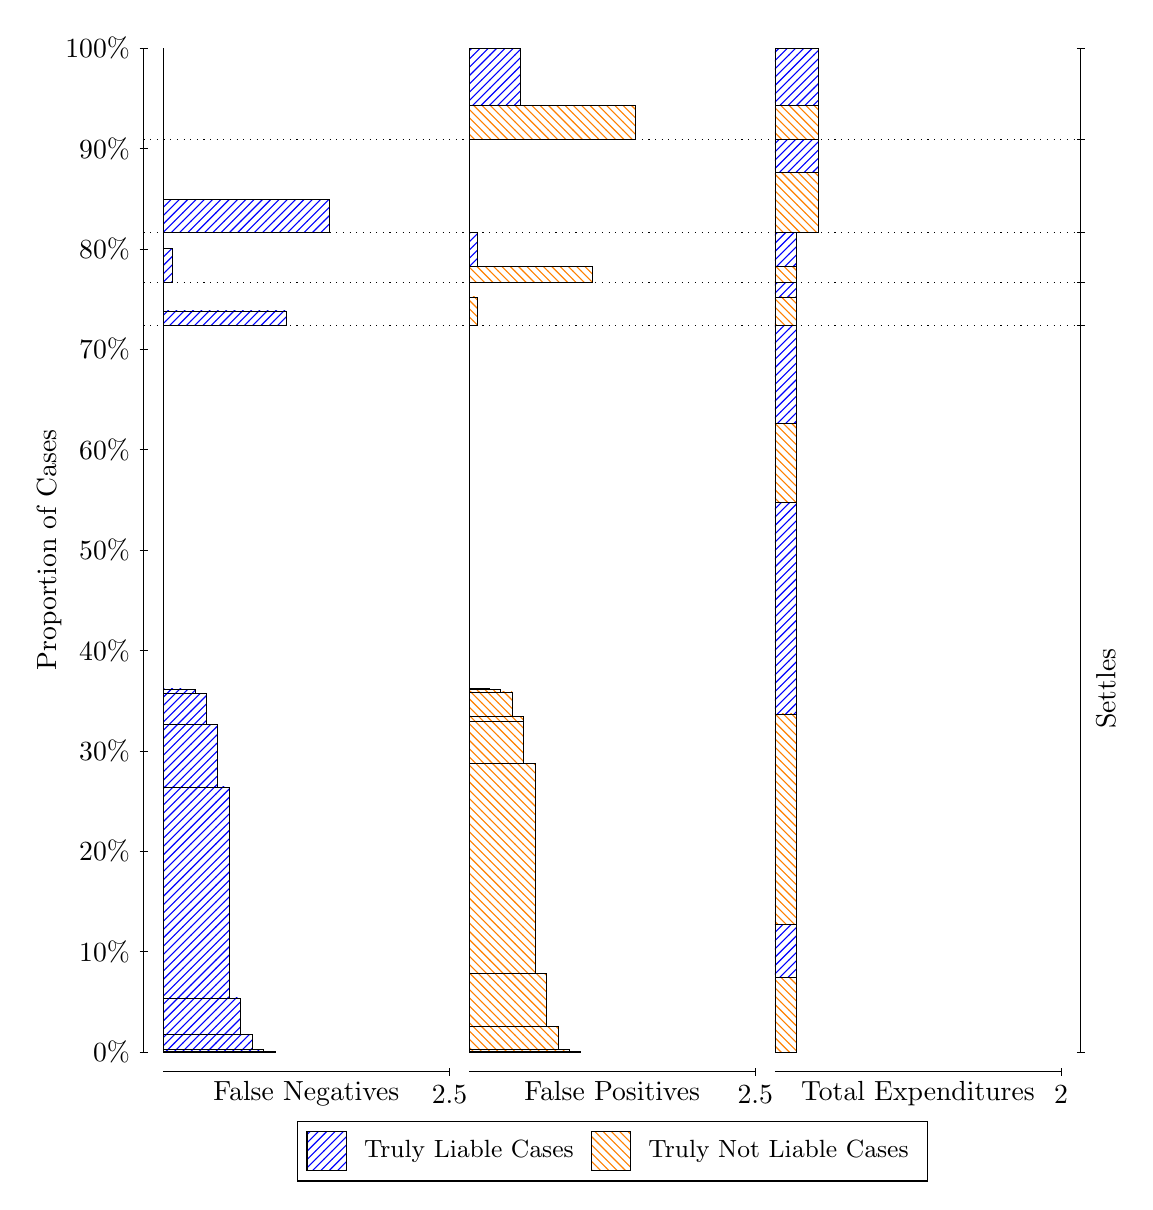
\begin{tikzpicture}
\draw[black, very thin] (1.5,1.75) -- (1.5,14.5);
\node[rotate=90, text=black, anchor=center] at (0.3, 8.125) {Proportion of Cases};
\draw[black, very thin] (1.45,1.75) -- (1.55,1.75);
\node[text=black, anchor=east] at (1.45, 1.75) {0\%};
\draw[black, very thin] (1.45,3.025) -- (1.55,3.025);
\node[text=black, anchor=east] at (1.45, 3.025) {10\%};
\draw[black, very thin] (1.45,4.3) -- (1.55,4.3);
\node[text=black, anchor=east] at (1.45, 4.3) {20\%};
\draw[black, very thin] (1.45,5.575) -- (1.55,5.575);
\node[text=black, anchor=east] at (1.45, 5.575) {30\%};
\draw[black, very thin] (1.45,6.85) -- (1.55,6.85);
\node[text=black, anchor=east] at (1.45, 6.85) {40\%};
\draw[black, very thin] (1.45,8.125) -- (1.55,8.125);
\node[text=black, anchor=east] at (1.45, 8.125) {50\%};
\draw[black, very thin] (1.45,9.4) -- (1.55,9.4);
\node[text=black, anchor=east] at (1.45, 9.4) {60\%};
\draw[black, very thin] (1.45,10.675) -- (1.55,10.675);
\node[text=black, anchor=east] at (1.45, 10.675) {70\%};
\draw[black, very thin] (1.45,11.95) -- (1.55,11.95);
\node[text=black, anchor=east] at (1.45, 11.95) {80\%};
\draw[black, very thin] (1.45,13.225) -- (1.55,13.225);
\node[text=black, anchor=east] at (1.45, 13.225) {90\%};
\draw[black, very thin] (1.45,14.5) -- (1.55,14.5);
\node[text=black, anchor=east] at (1.45, 14.5) {100\%};

\draw[black, very thin] (13.4,1.75) -- (13.4,14.5);
\draw[black, very thin] (13.35,1.75) -- (13.45,1.75);
\node[anchor=west] at (13.35, 1.75) {};
\draw[black, very thin] (13.35,10.978) -- (13.45,10.978);
\node[anchor=west] at (13.35, 10.978) {};
\draw[black, very thin] (13.35,11.526) -- (13.45,11.526);
\node[anchor=west] at (13.35, 11.526) {};
\draw[black, very thin] (13.35,12.157) -- (13.45,12.157);
\node[anchor=west] at (13.35, 12.157) {};
\draw[black, very thin] (13.35,13.343) -- (13.45,13.343);
\node[anchor=west] at (13.35, 13.343) {};
\draw[black, very thin] (13.35,14.5) -- (13.45,14.5);
\node[anchor=west] at (13.35, 14.5) {};

\draw[black, very thin, pattern color=blue, pattern=north east lines] (1.75,1.75) rectangle (3.167,1.7578);
\draw[black, very thin, pattern color=blue, pattern=north east lines] (1.75,1.7578) rectangle (3.0217,1.7788);
\draw[black, very thin, pattern color=blue, pattern=north east lines] (1.75,1.7788) rectangle (2.8763,1.9746);
\draw[black, very thin, pattern color=blue, pattern=north east lines] (1.75,1.9746) rectangle (2.731,2.436);
\draw[black, very thin, pattern color=blue, pattern=north east lines] (1.75,2.436) rectangle (2.5857,5.1159);
\draw[black, very thin, pattern color=blue, pattern=north east lines] (1.75,5.1159) rectangle (2.4403,5.9076);
\draw[black, very thin, pattern color=blue, pattern=north east lines] (1.75,5.9076) rectangle (2.295,6.3045);
\draw[black, very thin, pattern color=blue, pattern=north east lines] (1.75,6.3045) rectangle (2.1497,6.3552);
\draw[black, very thin, pattern color=blue, pattern=north east lines] (1.75,6.3552) rectangle (2.0043,6.3623);
\draw[black, very thin, pattern color=orange, pattern=north west lines] (1.75,6.3623) rectangle (1.75,10.978);
\draw[black, very thin, pattern color=blue, pattern=north east lines] (1.75,10.978) rectangle (3.3123,11.163);
\draw[black, very thin, pattern color=orange, pattern=north west lines] (1.75,11.163) rectangle (1.75,11.526);
\draw[black, very thin, pattern color=blue, pattern=north east lines] (1.75,11.526) rectangle (1.859,11.958);
\draw[black, very thin, pattern color=orange, pattern=north west lines] (1.75,11.958) rectangle (1.75,12.157);
\draw[black, very thin, pattern color=blue, pattern=north east lines] (1.75,12.157) rectangle (3.8573,12.576);
\draw[black, very thin, pattern color=orange, pattern=north west lines] (1.75,12.576) rectangle (1.75,13.343);
\draw[black, very thin, pattern color=orange, pattern=north west lines] (1.75,13.343) rectangle (1.75,13.774);
\draw[black, very thin, pattern color=blue, pattern=north east lines] (1.75,13.774) rectangle (1.75,14.5);
\draw[black, very thin, pattern color=orange, pattern=north west lines] (5.6333,1.75) rectangle (7.0503,1.7563);
\draw[black, very thin, pattern color=orange, pattern=north west lines] (5.6333,1.7563) rectangle (6.905,1.7817);
\draw[black, very thin, pattern color=orange, pattern=north west lines] (5.6333,1.7817) rectangle (6.7597,2.0743);
\draw[black, very thin, pattern color=orange, pattern=north west lines] (5.6333,2.0743) rectangle (6.6143,2.7497);
\draw[black, very thin, pattern color=orange, pattern=north west lines] (5.6333,2.7497) rectangle (6.469,5.4159);
\draw[black, very thin, pattern color=orange, pattern=north west lines] (5.6333,5.4159) rectangle (6.3237,5.9512);
\draw[black, very thin, pattern color=orange, pattern=north west lines] (5.6333,5.9512) rectangle (6.3237,6.011);
\draw[black, very thin, pattern color=orange, pattern=north west lines] (5.6333,6.011) rectangle (6.1783,6.3241);
\draw[black, very thin, pattern color=orange, pattern=north west lines] (5.6333,6.3241) rectangle (6.033,6.3585);
\draw[black, very thin, pattern color=orange, pattern=north west lines] (5.6333,6.3585) rectangle (5.8877,6.3654);
\draw[black, very thin, pattern color=blue, pattern=north east lines] (5.6333,6.3654) rectangle (5.6333,10.978);
\draw[black, very thin, pattern color=orange, pattern=north west lines] (5.6333,10.978) rectangle (5.7423,11.34);
\draw[black, very thin, pattern color=blue, pattern=north east lines] (5.6333,11.34) rectangle (5.6333,11.526);
\draw[black, very thin, pattern color=orange, pattern=north west lines] (5.6333,11.526) rectangle (7.1957,11.725);
\draw[black, very thin, pattern color=blue, pattern=north east lines] (5.6333,11.725) rectangle (5.7423,12.157);
\draw[black, very thin, pattern color=orange, pattern=north west lines] (5.6333,12.157) rectangle (5.6333,12.924);
\draw[black, very thin, pattern color=blue, pattern=north east lines] (5.6333,12.924) rectangle (5.6333,13.343);
\draw[black, very thin, pattern color=orange, pattern=north west lines] (5.6333,13.343) rectangle (7.7407,13.774);
\draw[black, very thin, pattern color=blue, pattern=north east lines] (5.6333,13.774) rectangle (6.2873,14.5);
\draw[black, very thin, pattern color=orange, pattern=north west lines] (9.5167,1.75) rectangle (9.7892,2.6926);
\draw[black, very thin, pattern color=blue, pattern=north east lines] (9.5167,2.6926) rectangle (9.7892,3.3708);
\draw[black, very thin, pattern color=orange, pattern=north west lines] (9.5167,3.3708) rectangle (9.7892,6.0439);
\draw[black, very thin, pattern color=blue, pattern=north east lines] (9.5167,6.0439) rectangle (9.7892,8.7315);
\draw[black, very thin, pattern color=orange, pattern=north west lines] (9.5167,8.7315) rectangle (9.7892,9.7312);
\draw[black, very thin, pattern color=blue, pattern=north east lines] (9.5167,9.7312) rectangle (9.7892,10.978);
\draw[black, very thin, pattern color=orange, pattern=north west lines] (9.5167,10.978) rectangle (9.7892,11.34);
\draw[black, very thin, pattern color=blue, pattern=north east lines] (9.5167,11.34) rectangle (9.7892,11.526);
\draw[black, very thin, pattern color=orange, pattern=north west lines] (9.5167,11.526) rectangle (9.7892,11.725);
\draw[black, very thin, pattern color=blue, pattern=north east lines] (9.5167,11.725) rectangle (9.7892,12.157);
\draw[black, very thin, pattern color=orange, pattern=north west lines] (9.5167,12.157) rectangle (10.062,12.924);
\draw[black, very thin, pattern color=blue, pattern=north east lines] (9.5167,12.924) rectangle (10.062,13.343);
\draw[black, very thin, pattern color=orange, pattern=north west lines] (9.5167,13.343) rectangle (10.062,13.774);
\draw[black, very thin, pattern color=blue, pattern=north east lines] (9.5167,13.774) rectangle (10.062,14.5);
\draw[black, dotted] (1.5,10.978) -- (13.4,10.978);
\draw[black, dotted] (1.5,11.526) -- (13.4,11.526);
\draw[black, dotted] (1.5,12.157) -- (13.4,12.157);
\draw[black, dotted] (1.5,13.343) -- (13.4,13.343);
\draw[black, very thin] (1.75,1.5) -- (5.3833,1.5);
\node[text=black, anchor=north] at (3.5667, 1.5) {False Negatives};
\draw[black, very thin] (5.3833,1.45) -- (5.3833,1.55);
\node[text=black, anchor=north] at (5.3833, 1.45) {2.5};

\draw[black, very thin] (5.6333,1.5) -- (9.2667,1.5);
\node[text=black, anchor=north] at (7.45, 1.5) {False Positives};
\draw[black, very thin] (9.2667,1.45) -- (9.2667,1.55);
\node[text=black, anchor=north] at (9.2667, 1.45) {2.5};

\draw[black, very thin] (9.5167,1.5) -- (13.15,1.5);
\node[text=black, anchor=north] at (11.333, 1.5) {Total Expenditures};
\draw[black, very thin] (13.15,1.45) -- (13.15,1.55);
\node[text=black, anchor=north] at (13.15, 1.45) {2};

\node[text=black, centered, rotate=90] at (13.72, 6.3638) {Settles};





\draw (7.449999999999999,1.5) node[draw=none] (baseCoordinate) {};
\begin{scope}[align=center]
        \matrix[scale=0.5, draw=black, below=0.5cm of baseCoordinate, nodes={draw}, column sep=0.1cm]{
            \node[rectangle, draw, minimum width=0.5cm, minimum height=0.5cm, pattern color=blue, pattern=north east lines] {}; &
            \node[draw=none, font=\small, text=black] (B) {Truly Liable Cases}; &
            \node[rectangle, draw, minimum width=0.5cm, minimum height=0.5cm, pattern color=orange, pattern=north west lines] {}; &
            \node[draw=none, font=\small, text=black] (B) {Truly Not Liable Cases}; \\
            };
\end{scope}

\end{tikzpicture}
\end{document}